\documentclass[twocolumn,10pt]{article}
\usepackage[greek,francais,english]{babel}
\usepackage[T1]{fontenc}
\usepackage[utf8]{inputenc}
\usepackage[top=2cm, bottom=2cm, left=1.5cm, right=1.5cm]{geometry}
\setlength{\columnsep}{1cm}
\usepackage[usenames,dvipsnames]{color}
\usepackage{graphicx}
%\usepackage{multicol}
\usepackage{eurosym} 
\usepackage{titlesec}
\usepackage[hang,small]{caption}
\renewcommand{\rmdefault}{ptm}
\newcommand\tet{\textgreek{tetraf'armakos} }
\titleformat{\section}{}{\thesection}{1em}{}
\titleformat{\subsection}{\it}{\thesubsection}{1em}{}
\titleformat{\paragraph}{\it}{theparagraph}{1em}{}
%================
\begin{document}
\title{\Huge \tet %en cas de problème avec cette fonte, ne pas hesiter à enlever le \tet en le commentant avec un % suivit d'un passage à la ligne
: Vegetation, atmosphere\\ and flight parameters monitoring} 
\author{Clément Javerzac-Galy \and{Denis Savoie}\\
\texttt{cansat2012@supop.fr}
\and{Zubair Iftikhar}
}
%\date{\today}
\date{}
\maketitle
 
\pagestyle{empty}
\thispagestyle{empty}
 
\begin{abstract}
    \begin{bfseries}
    \par \small The \tet \footnote{pronounce tetrapharmakos} is a Cansat project of the \textit{Proton-thérapeutes} team for the second participation of the Institut d'Optique \textit{Graduate School} to the \textit{C'Space} competition co-organized by Planète-Sciences and the CNES. 
    \par \small This space probe as a homemade embedded module to detect chlorophyll. It will also make an atmospheric sounding and position tracking during its fall.
    \par \small We hope these complementary studies could help to determine the chance of life on an Earth-like exoplanet.
     \end{bfseries}
\end{abstract}
\section{INTRODUCTION}%=========================================
    \par First of all, we need to precise that a Cansat is not really a satellite contained in a can. Indeed it will only fall instead of enter in any orbit. Then it is actually a space probe.
    \par We are making the \tet in order to participate to the competition a Cansat competition co-organized by \textit{Planète-Sciences} and the \textit{CNES} : the C'Space 2012. It have to fulfill 2 missions, one of which is free. For the imposed mission, we decided to do an atmospheric sounding. And our Fourier Optics professor Jean Taboury suggested us to make an NDVI measurement for the free mission.
    \par In addition to these 2 missions, another aspect of our work is to build a whole system. That means a probe that can be contained in 33 cL, fast enough to acquire a lot of informations, electrically autonomous, entirely automatic during the flight and finally resistant to a 200m fall --- using a parachute, of course.
\section{Context of development}%================================
    \subsection{Club}%&&&
    \par The \textit{Proton-thérapeutes} team is composed of 3 first-year MSc students at the Institut d'Optique \textit{Graduate School}. The first time our school participated to the Cansat competition was in 2011. This project has been initiated by Jean-Marie Feybesse, IT professor at Paris XI. But unfortunately, this team\footnote{Archimede, leaded by Sébastien Giudicelli} didn't reached the last step of competition because of logistic issues.
    \par As the previous team, we are 3. This number is too little not to be aware of the work of the whole team. Each member has not a specific work. Nevertheless some leadings have emerged, then we can describe the team as the following list:
    \begin{itemize}
        \item Clément: mechanics and electronic circuits designer
        \item Denis: electronics and cameras implementation
        \item Zubair: sensors implementation and parachute design
    \end{itemize}
\begin{figure}[!h]
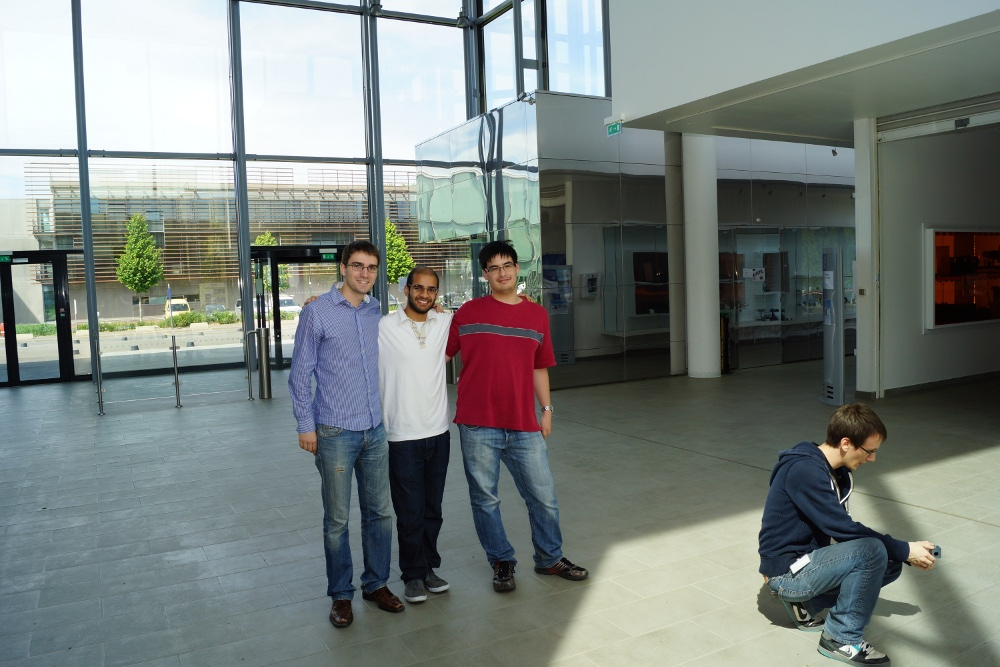
\includegraphics[scale=.25]{equipe.jpg}
\caption{\textit{Proton-thérapeutes} team. From left to right : Clément, Zubair and Denis. A friend of ours is holding the imagery system}
\end{figure}
    \subsection{Work plan}%&&&
    \par The team has been formed in November, our first job was to find the best electronic parts for our applications and draw a quick draft of the \tet organisation. Then we tested all the components we received. These preliminary tests went right but they have been done on a breadboard. 
    
    \par In April we decided to face non-electronic issues while we were trying to minimize the hardware connections. In May we felt good with non-electronic parts, our main job is now to get cameras working as we want.
    
    \par We have planned to have electronic unity with cameras and sensors in June, and input all the parts in plastic tube. Then we believe we will be ready in July to do our first test flight.
    
\section{DEFINITION OF THE MISSIONS}%================================
    \subsection{Proposed mission : Atmospheric sounding}%&&&
        \par We chose to measure the temperature, the humidity and the pressure during the fall of our cansat thanks to two electronic captors : the BMP085 that measures the temperature and the pressure, and the DHT22 that measures the temperature and the humidity.
        \par Measurements are made every two seconds, which is the refreshment rate of the used captors, and the requirement of the mission.
    \subsection{Free mission : chlorophyll detection}%&&&
        \par In this mission, we detect active chlorophyll by multispectral imagery.
        \paragraph*{Chlorophyll spectrum} Chlorophyll absorbs much red, and emits in near infrared, as we can see on Fig~\ref{spectrum_chl}.
        \begin{figure}[!h]
        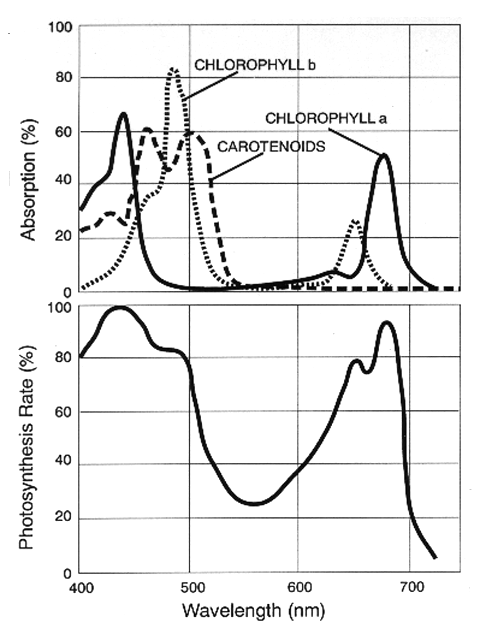
\includegraphics[scale=.4]{Par_action_spectrum.png}
        \caption{Absorption and fluorescence spectrum of chlorophyll}
        \label{spectrum_chl}
        \end{figure}
        \par So we use this by taking two pictures of the same scene, one in a red spectral band, the other in a near infrared spectral band. We then calculate the Normalized Difference Vegetation Index(NDVI) with this formula :
         \[ \textrm{NDVI} = \frac{\textrm{RED}-\textrm{NIR}}{\textrm{RED}+\textrm{NIR}} \]
        \paragraph*{Detection system} The images in red and in NIR bands are taken by two CCD. In order to detect red on one CCD, and NIR on the other, we use a cold mirror and filters. The hot mirror transmits most of visible light, and reflects most of infrared. Just like the chlorophyll its reflection and transmission spectrum cuts around $700\textrm{nm}$.
        \par  Just before the CCD, we put filters because the hot mirror reflects a part of the visible light (by eye observation about as much as a regular glass, about 4 \%) and it transmits all the visible light and not only the red part. The use of the hot mirror allows to keep a better part of the flux for both bands than a simple beam splitter, and allows to cut infrared for the red detector. 
        \par Before the hot mirror, we use a camera lens to form the image on both CCD, for instance we used a simple lens. The schematic of the optical system is given on Fig~\ref{sch_opt}.
        \begin{figure}[!h]
        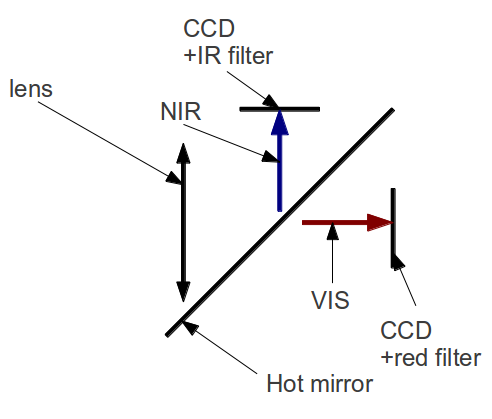
\includegraphics[scale=.5]{sch_opt.png}
        \caption{Schematic of the imagery system}
        \label{sch_opt}
        \end{figure}
        \begin{figure}[!h]
        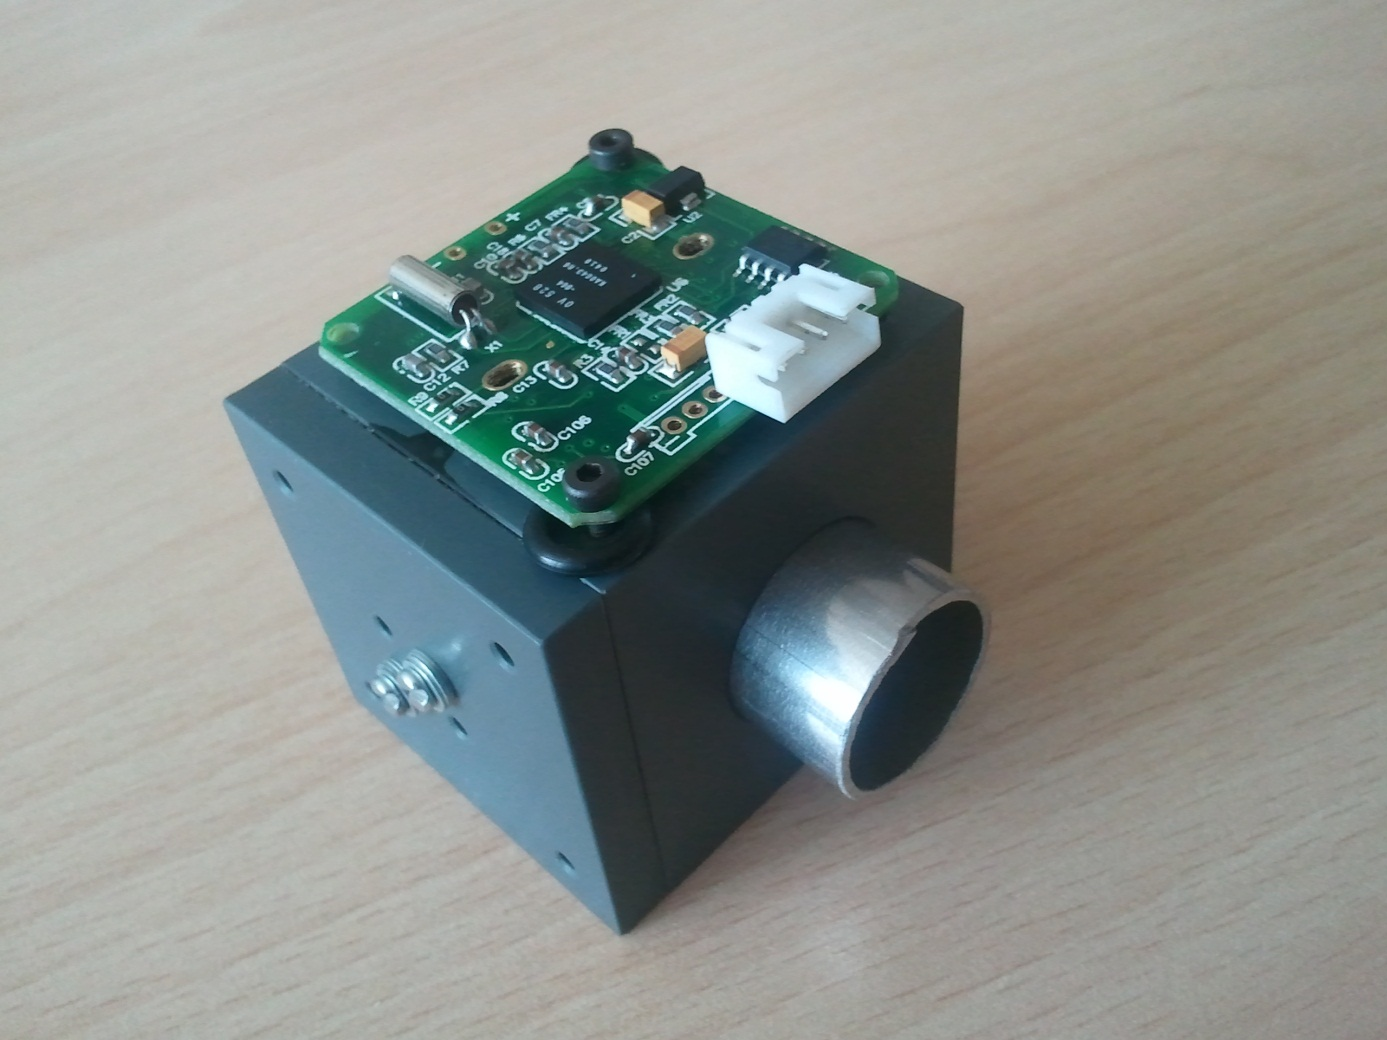
\includegraphics[scale=.5]{cube.png}
        \caption{Photograph of the assembled imagery system}
        \label{img_cube}
        \end{figure}
        
        \begin{figure}[!h]
        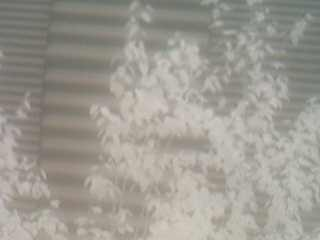
\includegraphics[scale=.7]{rehu.jpg}
        \caption{\small A picture taken by our system in NIR}
        \label{rehu}
        \end{figure}
    \subsection{Additional measurements}%&&&
    \par We also track the position and the speed of the cansat thank to an accelerometer and a GPS module. It will be useful to fit pressure measurements with a model. 
\section{CANSAT ARCHITECTURE}%====================================
    \subsection{Electrical architecture}%&&&
    \par The electrical architecture of the \tet is based on 2 Arduino Mini which load ATmega328 micro-controller. Because of an instable serial connection we found wiser to use each Arduino for a camera instead of putting the 2 cameras on the same. Then the architecture we decided is not the more elegant we would hope to have at first, it is described below:
    \begin{itemize}
    \item Arduino \no 1 (micro-controller)
        \begin{itemize}
        \item $\mu$CAM \no 1 (camera)
        \item DHT22 (humidity, temperature sensor)
        \item BMP085 (pressure, temperature sensor)
        \end{itemize}
        
    \item Arduino \no 2 (micro-controller)
        \begin{itemize}
        \item $\mu$CAM \no 2 (camera)
        \item ADXL335 (accelerometer)
        \item GPS module
        \end{itemize}
        
    \item Xbee Pro (radio communication module)
    \end{itemize}
    
    \par The cameras embedded are able to store an image in cache to send it on demand by a serial connection. We can use a software serial communication instead of a real hardware UART, which we do with the XBee and the GPS, but in the case of the camera, we did not manage to make the camera detect the highest baudrate (115200 bauds), so we preferred to use hardware UART for both cameras.
    
    
    \subsection{Mechanical parts}%&&&
    \par There are 3 main mechanical parts in the \tet :  the cameras cube, the parachute and the tube.
    \par The cameras we decided to use were shipped with their own lens. But this part was too large to be used in a cansat, especially when we need 2 cameras. Thus we have unmounted these parts to use a unique lens. We designed a cube to stabilize the position of each part. By the way we put a place to set the hot mirror.
    
    \par We will try to take the most photographs we can during the flight. We also made a parachute to limit the speed of the \tet to the \textit{minimum} autorised by the rules. It has the shape of a cross, composed of 5 squares. To determine the total surface we compute
    \[ S=\frac{2\ mg}{\rho\ C_{x}V_{L}^2} \]
    with the mass $m=0.3$ kg, the gravitational acceleration $g=9.8$ m/$\textrm{s}^{-2}$, air density $\rho=1.2 \textrm{ kg/m}^3$, the drag coefficient $C_{x}=1$ and the speed we want $V_{L}=2$ m/s. We found a surface about $S=1.5 \textrm{ m}^2$
    
    \par Last but not least, the tube in which we will put all the components is obviously an important mechanical part, but it is a simple part. The Archimede team has given us a plastic tube. We have also made some circle by cutting PCB. And we have found spindles in brass to organize the space inside the can.
    \subsection{Telemetry}
    \par Datas are sent all along the flight thank to the XBee. We use the XBee as a simple serial cable replacement. 
    \par During the flight, several type of data are to be transmitted. Datas collected from atmosphere captors, accelerometer and GPS are sent as plain text. Photographs are sent as binary packages. In order to manage all those datas, we use a header system. Plain text data packages are expected to be one line long and end by a carriage return. Binary package headers contain the length of the package. 
    \par Since there is two micro-controllers, and that each of them as datas to transmit, the XBee is shared by the two, and since most of the volume of datas are pictures, sharing of the XBee is cadenced by the pictures taken : when a picture is taken by both cameras,  one of the Arduino begins to transmit the full picture (in several packages), then all its buffered text datas. Then the other Arduino does the same.
    \subsection{Flight algorithm}
    \par Cameras are powered off during until the beginning of the fall in order to spare batteries. When the beginning of flight signal is given, cameras are powered on and initialized and all captors begin to make measurements. 
    \par Atmosphere captors make measurement every two seconds, while accelerometer and GPS make measurement every seconds. The datas of Atmospheric captors, accelerometers and GPS are buffered until they are sent as described above. Picture are taken as fast as possible, that is as fast as pictures from both cameras can be taken simultaneously and both sent. Each camera can buffer one image, and so it can be kept until it is transmitted.
    \par On landing, the program goes on as it did during the flight for several seconds, then cameras are powered off and all transmissions are stopped.
    
    \subsection{Budgets}
    \begin{table}[!h]
    \centering
\begin{tabular}{||l|l|l|l||}
\hline
& Qtt & Total (\euro) & Description \\ \hline
Arduino Mini V04 & 2 & 34,20 & microcontrolers \\ \hline
Mini-USB adapter & 1 & 15,00 &  \\ \hline
BMP085 & 1 & 18,50 & pressure, temperature\\ \hline
RHT22 & 1 & 15,00 & humidity, temperature\\ \hline
ADXL335 & 1 & 22,46 & accelerometer\\ \hline
GPS & 1 & 28,00 & GPS\\ \hline
XBee Pro & 2 & 71,52 & data transmission\\ \hline
XBee Dongle USB & 1 & 20,58 & USB adapter\\ \hline
$\mu$CAM & 2 & 112,42 & camera\\ \hline
Mechanic &  & 0,00 & \\ \hline
Optic &  & 0,00 & \\ \hline \hline
TOTAL &  & 337,68 & \\ \hline
\end{tabular}
    \caption{\tet components prices}
\end{table}
\section{CONCLUSION}
\par After learning about the difficulties that appears when we carry such a project, we have know finished the hardware electronic part, and have just to solder definitive electric connections here and there. The big part of the mechanical structure is now built (we have a tube and the supports are built). 
\par We have yet to put all the components in it. We can tested every electronic components except the cameras, with which we took picture on a computer with a program of our own, and made work almost everything on a Arduino, but we still only have obtained corrupted image files. Before the flight, we have to definitively assemble all the parts of the \tet, figure out the problem with the camera, finish the programming and test it all.
\section*{ACKNOWLEDGEMENT}
We gratefully acknowledge: 
\begin{itemize}
\item Jean-Marie Feybesse, for his advice, direction and enthusiasm.
\item Thierry Avignon and Cedric Lejeune from the Institut d'Optique Service des Traveaux Pratiques, for helping us all along for all our homemade parts, in electronics, mechanics and optics.
\item Jean Taboury for the idea for our mission and his advices.
\item All the pedagogic team of the electronic labworks at the Institut d'Optique
\item The Atelier de Mécanique of the Institut d'Optique for the higher precision mechanical parts.
\item The Institut d'Optique that allowed us to carry this project, funded it, provided its tools, and made it all possible.
\item Martin Pertenaïs (1st year MSc), for helping us with optical design.
\item Lionel, from Snootlab, that helped us to choose the right material for programming the arduino.
\end{itemize}
\section*{Credits}
\begin{itemize}
\item \small Fig~\ref{spectrum_chl} : John Whitmarsh and Govindjee CC-BY-SA-2.0.
\end{itemize}
%\begin{thebibliography}{9}
  % la biblio
%\end{thebibliography}
\end{document}

